
\section{انگیزه‌ی پژوهش و صورت  مسئله}
%\begin{latin}
%VIII. CURRENT STATUS AND PERSPECTIVE
%Actor languages have been used for parallel and dis- tributed computing in the real world for some time (e.g. Charm++ for scientific applications on supercomputers, Er- lang for distributed applications). In recent years, interest in actor-based languages has been growing, among researchers as well as practitioners. This interest is triggered by emerg- ing programming platforms such as multicore computers, cloud computers, Web services, and sensor networks. In some cases, such as cloud computing, web services and sensor networks, the Actor model is a natural programming model because of the distributed nature of these platforms. As multicore architectures are scaled, multicore computers will also look more more like the traditional multicomputer platforms. This is illustrated by the prototype, 48-core Single-Chip Cloud Computer (SCC) developed by Intel [36]. However, the argument for using actor-based programming languages is not simply that they provide a good match for representing computation on a variety of parallel and dis- tributed computing platforms. The point is that by extending object-based modeling to concurrent agents, actors provide a good starting point for simplifying the task of parallel (distributed, mobile) programming.
%\end{latin}
%(از مقاله‌ی آقا ۲۰۱۰)
در سال‌های اخیر در روند افزایش سرعت پردازنده‌ها تغییر قابل ملاحظه‌ای به وجود آمده است. در سالهای گذشته افزایش سرعت پردازنده‌ها به معنی افزایش فرکانس چیپ‌های پردازنده بوده است، بدین مفهوم که تقریبا با گذشت هر ۲ سال،‌ سرعت پردازشی پردازنده‌ها حدودا ۱/۵ برابر شده‌اند. این روند در شکل 
\ref{fig:CPU_Trend}
تا حدود سال ۲۰۰۵ قابل مشاهده است. در این روند شاهد افزایش بدون توقف سرعت پردازنده‌ها بوده‌ایم. همان طور که شکل نشان می‌دهد، در ادامه‌ی این این روند شاهد توقف افزایش سرعت پردازش بوده‌ایم. با وجود این توقف افزایش سرعت، تعداد ترانزیستور‌های پردازنده‌ها طبق روند قبلی افزایش یافته است. این تغییر به این معناست که در زمینه‌ی قدرت پردازش پردازنده‌ها، افزایش تعداد هسته‌های پردازشی جایگزین افزایش سرعت پردازشی هسته‌ها شده است. با توجه به این تغییر در روند بهبود سرعت پردازنده‌ها، نقش طراحی برنامه در افزایش كارایی آن از نظر سرعت اجرا پررنگ‌تر شده است. در این وضعیت عامل اصلی تاثیر گذار بر سرعت اجرای برنامه، تعداد فرایندهای همروند آن می‌باشد. با افزایش همروندی، كارایی سیستم می‌تواند تا میزان محدودی افزایش پیدا کند. رویكرد معمول برای افزایش همروندی سیستم‌ها كه در پژوهش‌های متعددی به آن پرداخته شده است اختصاص فرایندها یا ریسمان های همروند برای انجام محاسبات مشابه می‌باشد. به عنوان مثال در یك برنامه تحت وب، تمام پردازش‌های مربوط به یك درخواست كه به یك وب سرور فرستاده می‌شود در یك ریسمان سرور اجرا می‌شود. در این رویكرد برای افزایش كارایی بیشتر تمركز روی تنظیم تعداد ریسمان‌های سرویس دهنده و نیز بهینه كردن زمانبندی تراكنش‌های پایگاه داده می‌باشد و بخشی از منطق دامنه كه برای سرویس دادن به درخواست اجرا می‌شود تاثیر چندانی بر كارایی ندارد. حوزه بحث این پژوهش، طراحی منطق دامنه برنامه مبتنی بر تبادل ناهمگام پیغام می‌باشد. ارتباط ناهمگام بین اشیاء برنامه منجر به ایجاد همروندی ریزدانه می‌گردد. در همروندی ریزدانه كه در این پژوهش به آن پرداخته خواهد شد، همروندی به عنوان خاصیتی در طراحی منطق دامنه در نظر گرفته می‌شود. در این رویكرد برای افزایش همروندی، به جای افزایش تعداد ریسمان‌هایی كه هر كدام یك كار مشابه را از ابتدا تا انتها انجام می‌دهند، منطق پردازش یك درخواست با استفاده از ارتباط ناهمگام اشیاء و همروندی ریزدانه طراحی می‌شود. برای پیاده‌سازی همروندی به جای استفاده از ریسمان‌ها، از روش تبادل ناهمگام پیغام استفاده خواهد شد. دلیل عدم استفاده از ریسمان‌ها یكی مشكلات ناشی از وجود حالت مشترك 
\LTRfootnote{Shared State} 
بین ریسمان‌ها است و دیگری این است كه آمیخته شدن كدهای مربوط به ریسمان با منطق دامنه‌ی برنامه مطلوب نمی‌باشد. هدف از انجام این پژوهش بررسی روش طراحی شیءگرای منطق دامنه بر اساس ایده‌ی ارتباط ناهمگام و همروندی ریزدانه و بررسی اثر آن در ویژگی‌های كیفی نرم‌افزار است. در این پژوهش، ویژگی‌های كیفی كارایی
\LTRfootnote{Performance} 
و تغییرپذیری
\LTRfootnote{Modifiability} 
برای بررسی انتخاب شده‌اند.
\begin{figure}
    \begin{center}
    \begin{tabular}{ c }
  	 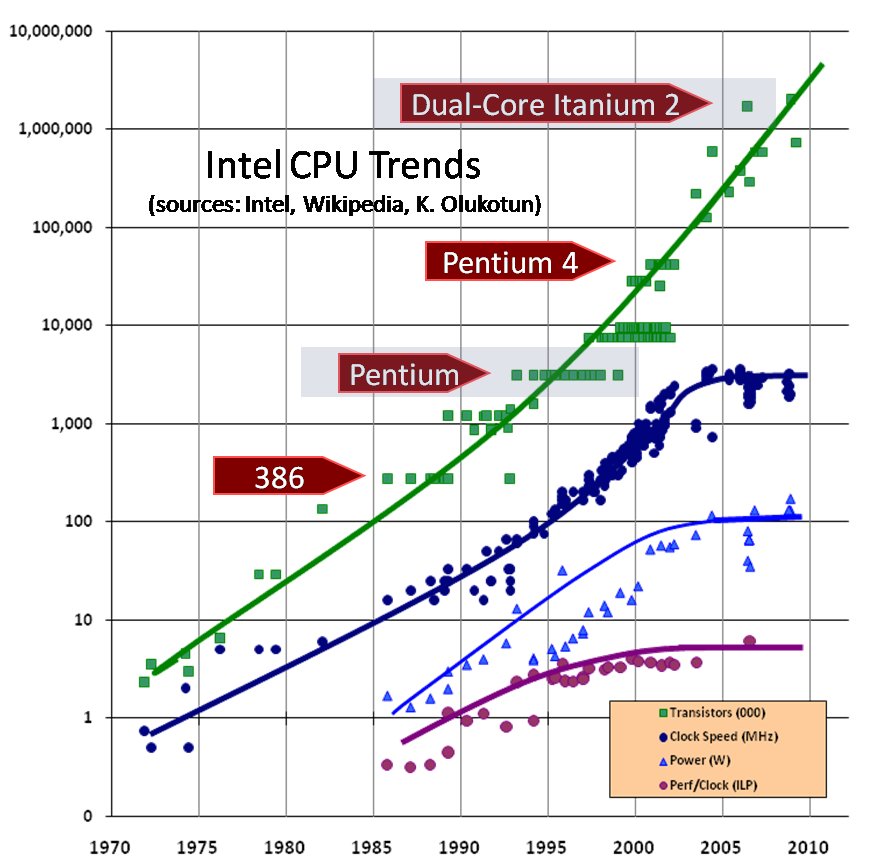
\includegraphics[width=12cm,height=8cm]{1-Introduction/Figures/Moore.png}
  \end{tabular}
  \end{center}
   \caption{\label{fig:CPU_Trend} روند افزایش سرعت پردازنده‌ها در سال‌های اخیر}
\end{figure}
%\section{صورت مسئله}
%موضوع این پژوهش بررسی روش طراحی منطق دامنه با استفاده از تبادل ناهمگام پیغام می‌باشد. در این روش اشیاء
%در طراحی به روش تبادل ناهمگام پیغام، علاوه بر نکات مربوط به طراحی شیءگرای ترتیبی، 
 
%\section{روش پژوهش}
%ارزیابی عملی با مطالعه‌ی موردی

\section{خلاصه‌ی دستاوردهای پژوهش}
برخی از دستاوردهای این پژوهش را می‌توان به این ترتیب برشمرد:
\begin{itemize}
\item  یک سیستم نمونه انتخاب شده و طراحی منطق دامنه‌ی آن به روش تبادل ناهمگام پیغام به طور کامل انجام شده است. ارائه‌ی روش طراحی به صورت مرحله‌ای و افزایشی باعث شده است تا بتوان از آن به صورت دستورالعملی برای طراحی همروند استفاده کرد. 
\item خروجی مهم پژوهش، روش‌ها و الگوهایی است که در این نوع طراحی کاربرد دارد. در هر الگوی استخراج شده، روش پیاده‌سازی در مدل اکتور و کاربردهای الگو از نظر منطق دامنه بررسی شده است. 
\item تجربیاتی که در طراحی‌های صورت گرفته کسب شده به صورت قابل استفاده‌ای ارائه شده است و مطالعه‌ی این تجربیات، خواننده را با نکات ظریف و  حساسی آشنا می‌کند که انجام طراحی به روش تبادل ناهمگام پیغام را بسیار ساده‌تر می‌کند.
\item در ارزیابی روش طراحی ناهمگام، خصوصیات کیفی این روش از جمله تغییرپذیری و کارایی آن با روش طراحی شیءگرای ترتیبی مقایسه شده و نشان داده شده است که علاوه بر اینکه از نظر تغییرپذیری دو روش قابل مقایسه هستند، طراحی به روش تبادل ناهمگام پیغام در مواردی باعث افزایش چشم‌گیر کارایی سیستم می‌گردد.
\end{itemize}
\section{ساختار پایان‌نامه}
برای بررسی این موارد، ساختار این متن در ۵ فصل تنظیم گردیده است:
\begin{strict_itemize}
\item  فصل ۲ به ارائه‌ی برخی پیش‌نیازهای طراحی به روش تبادل ناهمگام پیغام می‌پردازد. مدل اکتور و کتابخانه‌ی اکتور اسکالا در این فصل معرفی شده‌اند.
\item در فصل ۳ پژوهش‌های مرتبط معرفی شده‌اند. الگوهای طراحی با اکتورها و نیز کاربردهای صنعتی رویکرد تبادل ناهمگام پیغام در این فصل بررسی شده‌اند. علاوه بر آن روش‌های طراحی منطق دامنه در برنامه‌نویسی شیءگرا به طور مختصر معرفی شده‌اند.
\item در فصل ۴ روش طراحی منطق دامنه با استفاده از تبادل ناهمگام مورد بررسی قرار گرفته. روش طراحی با انتخاب یک سیستم نمونه و بسط روش طراحی آن ارائه شده و در پایان الگوها و نکات مهم طراحی استخراج شده‌اند. علاوه بر این، معیارهای کیفی سیستم طراحی شده با رویکرد تبادل ناهمگام بررسی شده و با همین‌ ویژگی‌ها در رویکرد طراحی ترتیبی مقایسه شده است.
\item نهایتا فصل ۵ به جمع‌بندی پژوهش، ارائه‌ی دستاوردها و ذکر تعدادی از جهت‌گیری‌های مرتبط برای پژوهش‌های آینده می‌پردازد.
\end{strict_itemize}
